\documentclass{beamer}

\usepackage[utf8]{inputenc}
\usepackage[T1]{fontenc}
\usepackage{amsmath}
\usepackage{bm}

\usepackage{tabularx}
\usepackage{graphicx}
\usepackage{epstopdf}
\usepackage{multirow}

\graphicspath{{../../images/}}

\usetheme{Madrid}
\usebeamercolor{sidebartab}
\usefonttheme{professionalfonts}


\title[M.Sc. Thesis 2015]{Spatial Summarization of Image Collections}
\author{Diego A. Ballesteros Villamizar}
\institute[ETHZ]{ETH Zürich}
\date{February 8th, 2016}

\DeclareMathOperator*{\argmin}{argmin}
\DeclareMathOperator*{\argmax}{argmax}

\AtBeginSection[]
{
  \begin{frame}<beamer>
    \frametitle{Outline}
    \tableofcontents[currentsection]
  \end{frame}
}

\begin{document}

\begin{frame}
  \titlepage
\end{frame}

\section{Augmented features}

\begin{frame}{Leftover question}
  \begin{itemize}
    \item Does using a feature matrix $\mathbf{X}' = \mathbf{X} \mid \mathbb{I}$ improve the results?
    \begin{table}
      \begin{tabular}{l|lllll}
        \hline
        & \multicolumn{5}{c}{K} \\
        \hline
        \multirow{5}{*}{L} & & 0 & 2 & 5 & 10 \\
        & 0 & $17.38 \pm 1.81$ & $18.75 \pm 2.95$ & $18.82 \pm 2.58$ & $18.91 \pm 2.40$ \\
        & 2 & $22.66 \pm 4.58$ & $28.53 \pm 4.36$ &&\\
        & 5 & $25.40 \pm 4.77$ && $31.59 \pm 2.38$ &\\
        & 10 & $31.13 \pm 2.92$ &&& $30.49 \pm 3.51$ \\
      \end{tabular}
    \end{table}
    \item Not really, the best score so far is $34.35 \pm 2.15$ with $\mathbf{X} = \mathbb{I}$.
    \item Running time is significantly slower, because of the increased number of features $M = N + 4$.
  \end{itemize}
\end{frame}

\section{Sampling the distribution}

\begin{frame}{Sampling from the model}
  \begin{itemize}
    \item Using the best model, i.e. without features and with $L = 5, K=5$.
    \item How does the resulting distribution look?
    \item How to use the distribution to recommend sets?
  \end{itemize}
\end{frame}

\begin{frame}{Exact sampling}
  \begin{itemize}
    \item With $N = 10$, it is possible to calculate the probabilities from the model for all $2^{10} = 1024$ possible sets.
    \item Evaluating the model on all sets $S \subseteq V$and then normalizing the probability distribution.
    \item Takes only seconds to evaluate.
  \end{itemize}
\end{frame}

\begin{frame}{Distribution of set size ($100k$ samples)}
  \begin{figure}
    \centering
    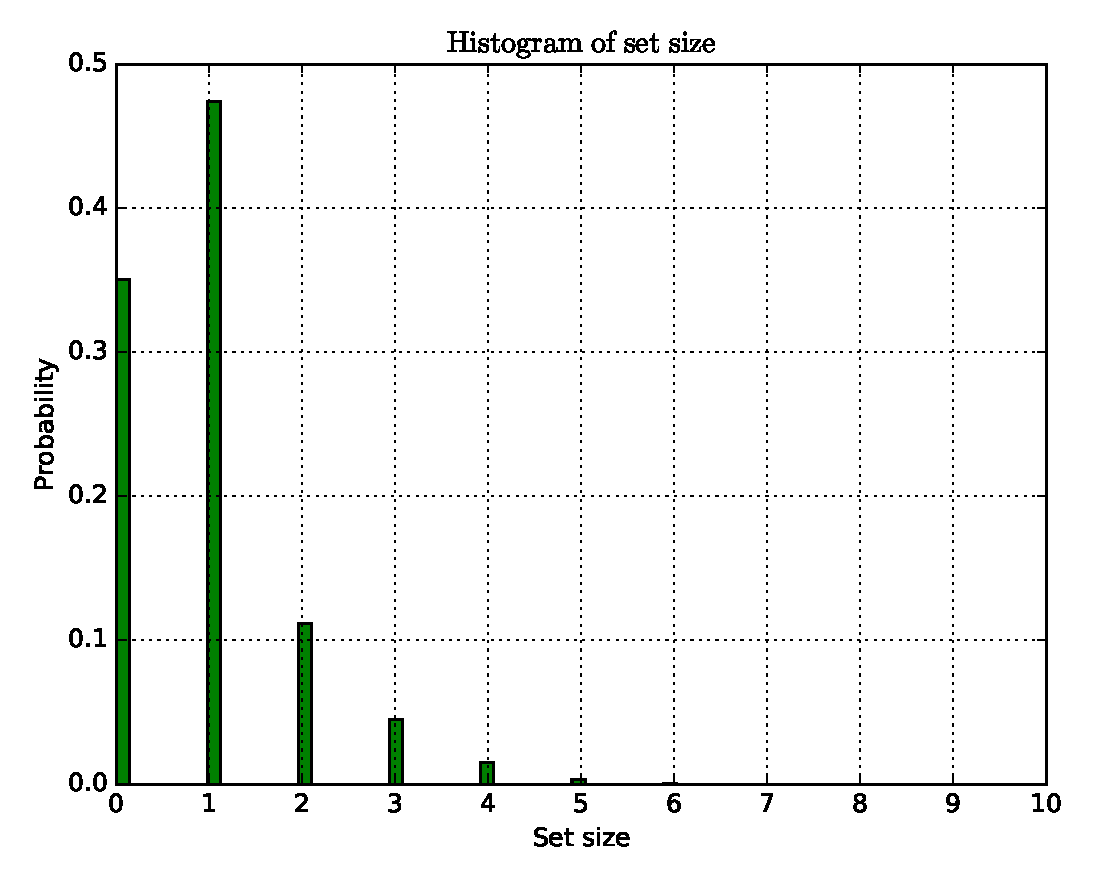
\includegraphics[height=0.8\textheight]{length_histogram_exact}
  \end{figure}
\end{frame}

\begin{frame}{Distribution of sets with $|S| = 2$ ($100k$ samples)}
  \begin{figure}
    \centering
    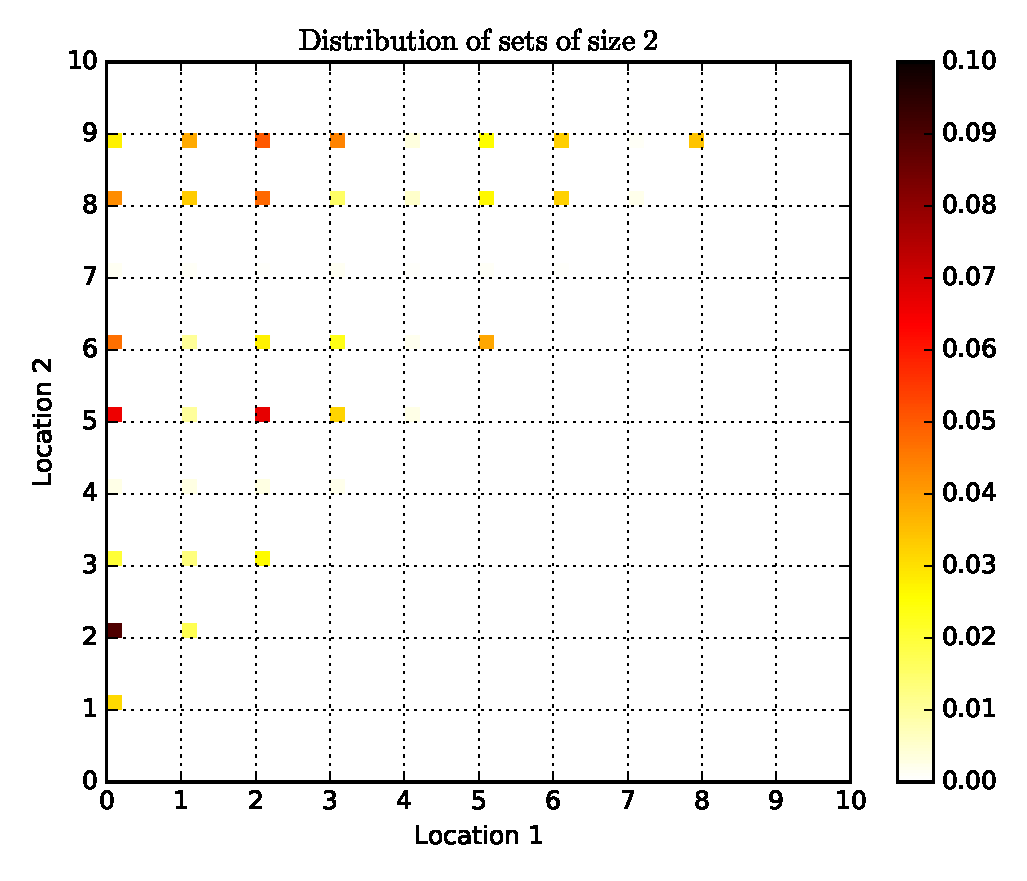
\includegraphics[height=0.8\textheight]{pairs_histogram_exact}
  \end{figure}
\end{frame}

\begin{frame}{Gibbs sampling}
  \begin{itemize}
    \item What about a method that scales? For example if $N = 30$, then there are $2^{30} = 1073741824$ sets.
    \item Gibbs sampling as presented in \cite{gotovos15sampling}.
    \item Run for $1M$ iterations, remove the first half of iterations are burn-in.
    \item Running time is a couple of minutes.
  \end{itemize}
\end{frame}

\begin{frame}{Distribution of set size ($100k$ samples)}
  \begin{figure}
    \centering
    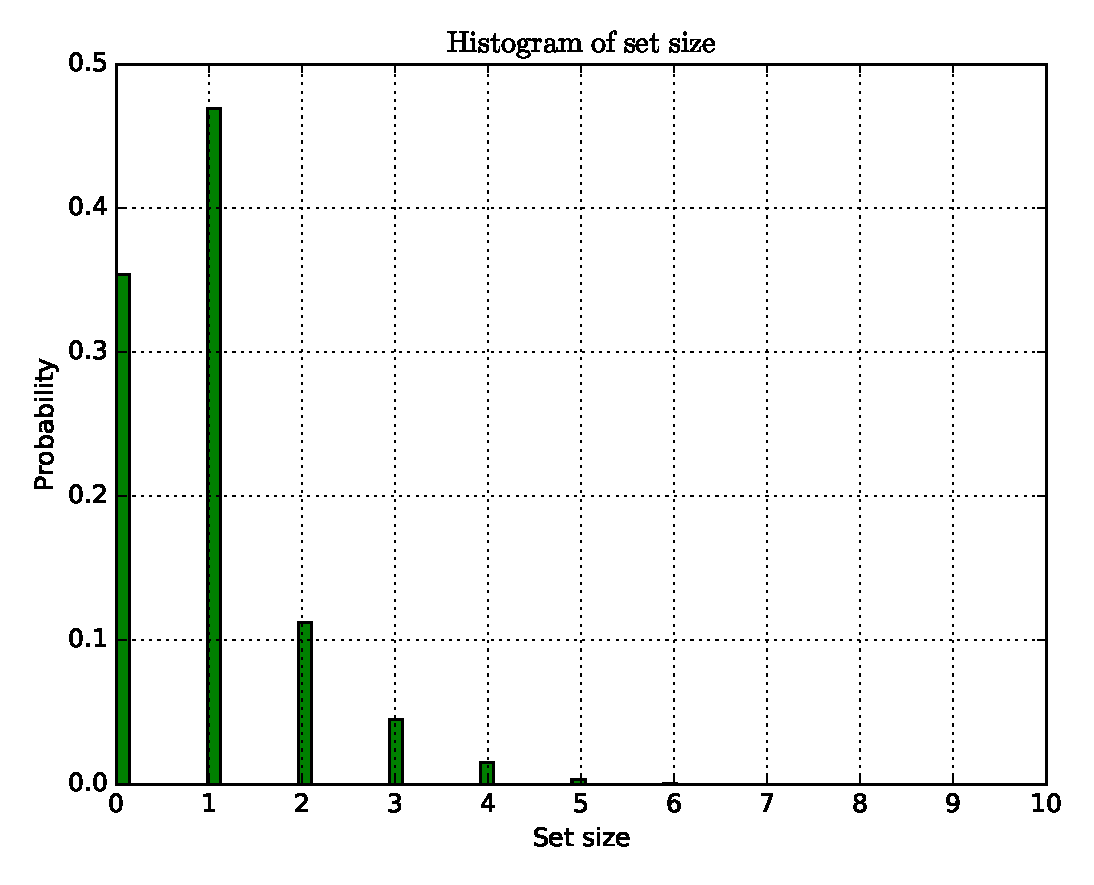
\includegraphics[height=0.8\textheight]{length_histogram_gibbs}
  \end{figure}
\end{frame}

\begin{frame}{Distribution of sets with $|S| = 2$ ($100k$ samples)}
  \begin{figure}
    \centering
    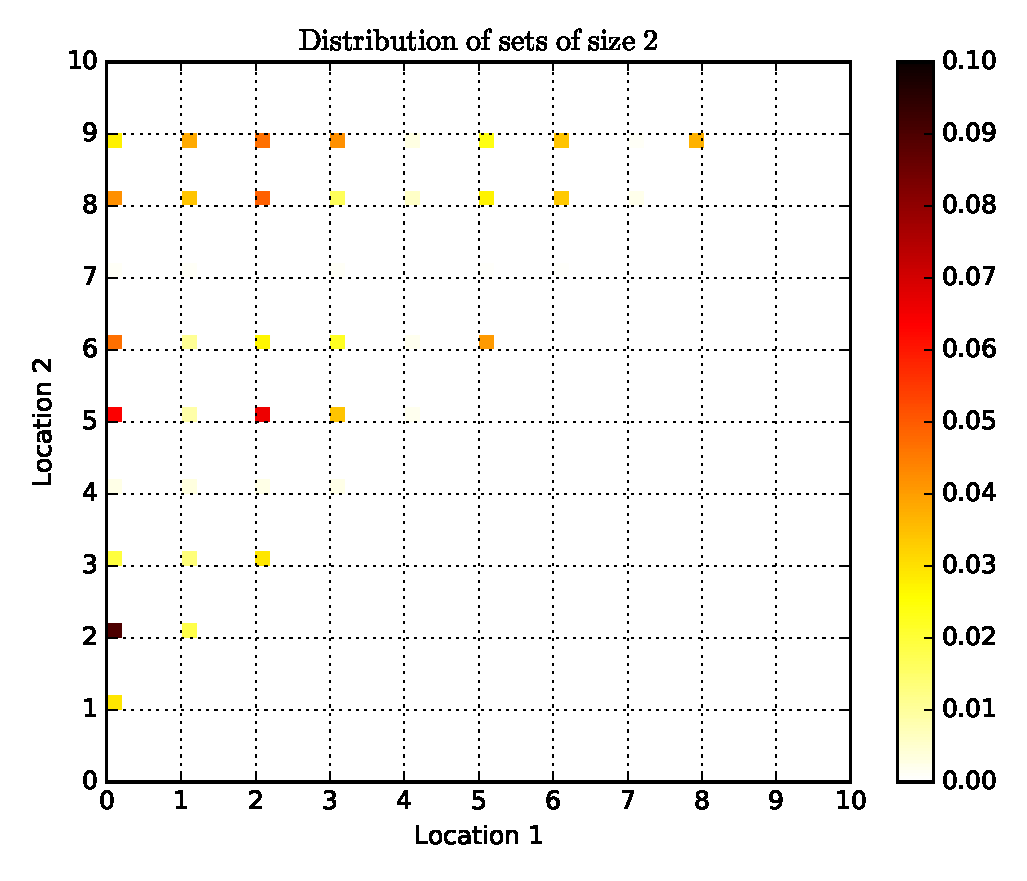
\includegraphics[height=0.8\textheight]{pairs_histogram_gibbs}
  \end{figure}
\end{frame}

\begin{frame}{Gibbs Sampling Performance}
  \begin{figure}
    \centering
    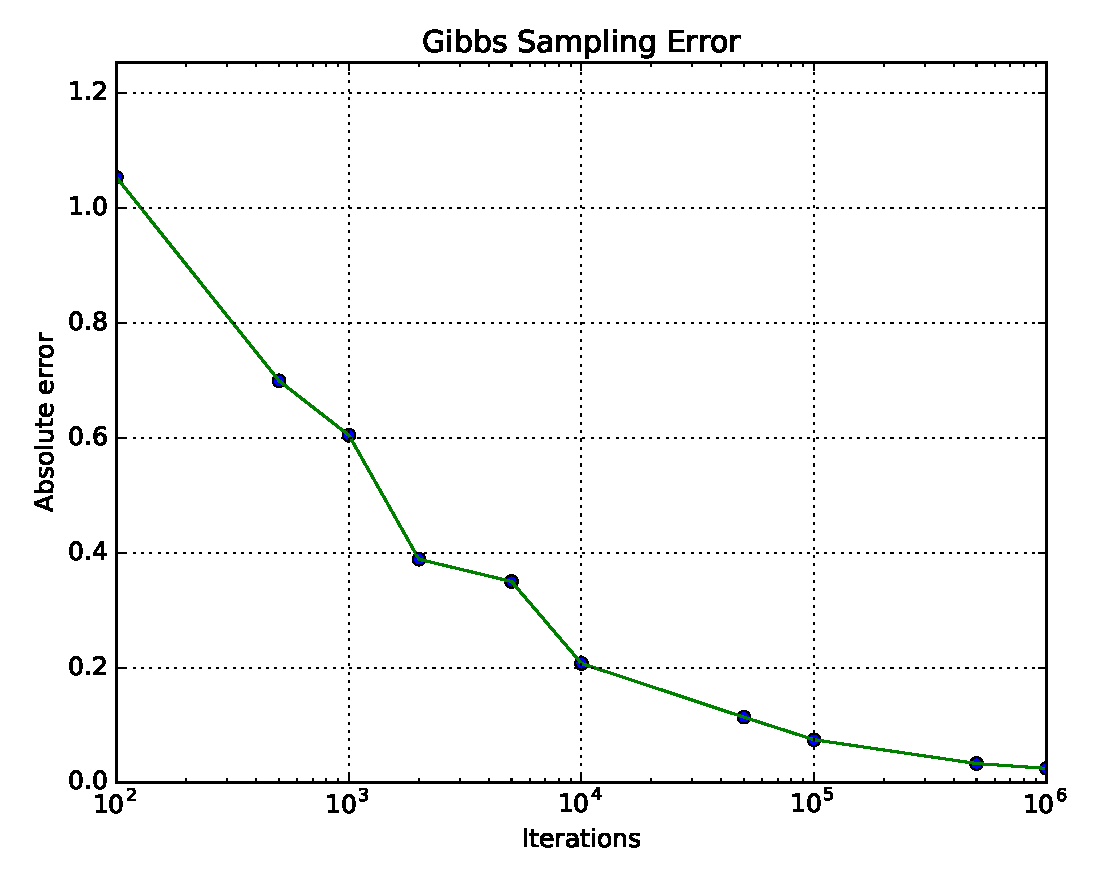
\includegraphics[height=0.8\textheight]{gibbs_performance}
  \end{figure}
\end{frame}

\section{Extending the location set}

\begin{frame}{More mean-shift clusters}
  \begin{itemize}
    \item Original dataset has over 160k photos.
    \item When clustered using mean-shift with a bandwidth of approximately 100m, there are over 2k clusters.
    \item Previous tests were done using the 10 top clusters according number of photos per cluster. This covered only over 30k photos.
    \item Does the approach scale if the number of clusters is increased?
    \item 50 clusters cover over 100k photos.
    \item 12k paths are present, in comparison there were 8k paths with 10 clusters.
  \end{itemize}
\end{frame}

\begin{frame}{Baselines}
  \begin{table}
    \centering
    \begin{tabular}{@{}lll@{}}
      \hline
      \textbf{Model} & \textbf{Accuracy} & \textbf{MRR} \\
      \hline
      Modular & $9.21 \pm 1.02$ & $27.00 \pm 1.01$ \\
      Markov & $19.72 \pm 1.23$ & $34.50 \pm 1.00$ \\
      \textbf{Markov with rejection} & $\mathbf{22.36 \pm 1.41}$ & $\mathbf{38.65 \pm 1.09}$ \\
      Proximity & $12.76 \pm 0.70$ & $27.71 \pm 0.88$ \\
      Proximity with rejection & $14.74 \pm 0.64$ & $31.34 \pm 1.14$ \\
      \hline
    \end{tabular}
  \end{table}
  \begin{itemize}
    \item Similar trend as with $N = 10$, Markov with rejection is the best model and it's significantly better than the modular model.
  \end{itemize}
\end{frame}

\begin{frame}{FLDC - Facility Location Diversity and Coherence}
  \begin{itemize}
    \item Use the best model from the case for $N = 10$.
    \item The model with a diversity term, i.e. submodular, and a coherence term, i.e. supermodular. Without features, i.e. $\mathbf{X} = \mathbb{I}$.
    \item Running on $k = 10$ folds, with a noise factor of 50.
    \item Latent dimensions are: $0 \leq L \leq 20, 0 \leq M \leq 20$.
  \end{itemize}
\end{frame}

\begin{frame}{Evaluation}
  \begin{table}
    \begin{tabular}{l|lllll}
      \hline
      & \multicolumn{5}{c}{K} \\
      \hline
      \multirow{5}{*}{L} & & 0 & 2 & 10 & 20 \\
      & 0 & $9.21 \pm 1.02$ & $16.24 \pm 1.43$ & $16.12 \pm 1.29$ & $16.44 \pm 1.77$\\
      & 2 & $12.09 \pm 1.36$ & $17.05 \pm 0.91$ &&\\
      & 10 & $12.94 \pm 1.39$ && $19.28 \pm 0.73$ &\\
      & 20 & $9.17 \pm 2.27$ &&& $\mathbf{21.53 \pm 1.24}$\\
    \end{tabular}
  \end{table}
  \begin{itemize}
    \item Model with diversity and coherence term has performance close to the markov model with rejection.
  \end{itemize}
\end{frame}

\begin{frame}{Distribution of set size ($100k$ samples)}
  \begin{figure}
    \centering
    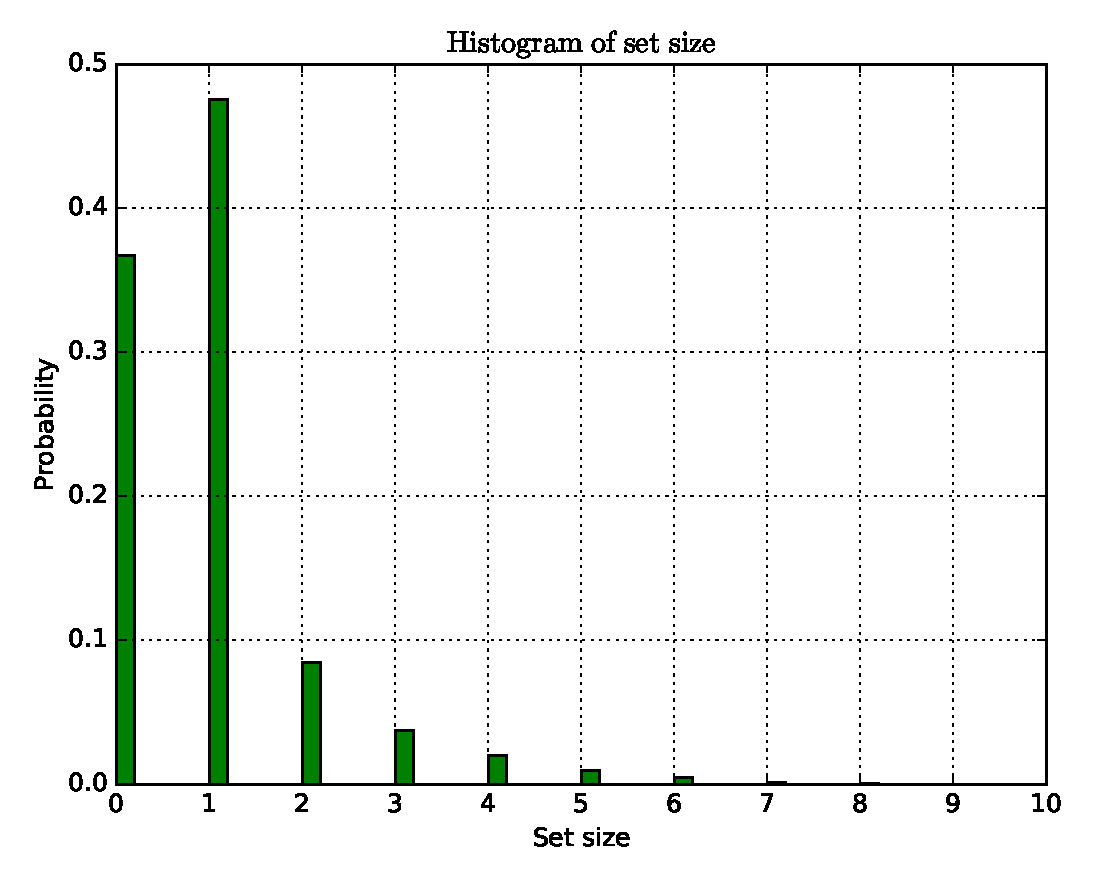
\includegraphics[height=0.8\textheight]{length_histogram_gibbs_50}
  \end{figure}
\end{frame}

\begin{frame}{Frequency of data}
  \begin{columns}
    \begin{column}{0.5\columnwidth}
      \begin{table}
        \centering
        \caption{Frequency of Item Sets}
        \begin{tabular}{ll}
          \hline
          Set & Frequency \\
          \hline
          $[0, 7]$ & 61\\
          $[27, 28]$ & 39\\
          $[13, 7]$ & 36\\
          $[11, 14]$ & 27\\
          $[0, 13]$ & 25\\
          $[2, 7]$ & 23\\
          $[10, 2]$ & 22\\
          $[25, 34]$ & 22\\
          $[2, 15]$ & 21\\
          $[10, 15]$ & 21\\
          \hline
        \end{tabular}
      \end{table}
    \end{column}
    
    \begin{column}{0.5\columnwidth}
      \begin{table}
        \centering
        \caption{Locations}
        \begin{tabular}{ll}
          \hline
          Index & Location \\
          \hline
          0 & Grossmünster \\
          2 & Bürkliterrasse \\
          7 & Fraumünster \\
          10 & Quaibrücke \\
          11 & Hauptbahnhof \\
          13 & Rathaus \\
          14 & Urania-Sternwarte \\
          15 & Bellevue \\
          25 & Frau Gerolds Garten \\
          27 & Zoo \\
          28 & Restaurant Masoala (Zoo) \\
          34 & Stadion Letzigrund \\
          \hline
        \end{tabular}
      \end{table}
    \end{column}
  \end{columns}
\end{frame}


\begin{frame}{References}
  \bibliographystyle{acm}
  \bibliography{../references}
\end{frame}

\end{document}
